% Vista preliminar del código fuente

%% LyX 2.0.0 created this file.  For more info, see http://www.lyx.org/.
%% Do not edit unless you really know what you are doing.
\documentclass[english]{article}
\usepackage[T1]{fontenc}
\usepackage[latin9]{inputenc}
\usepackage{float}
\usepackage{textcomp}
\usepackage{amstext}
\usepackage{graphicx}

\makeatletter

%%%%%%%%%%%%%%%%%%%%%%%%%%%%%% LyX specific LaTeX commands.
%% Binom macro for standard LaTeX users
\newcommand{\binom}[2]{{#1 \choose #2}}

%% Because html converters don't know tabularnewline
\providecommand{\tabularnewline}{\\}

%%%%%%%%%%%%%%%%%%%%%%%%%%%%%% Textclass specific LaTeX commands.
\newenvironment{lyxcode}
{\par\begin{list}{}{
\setlength{\rightmargin}{\leftmargin}
\setlength{\listparindent}{0pt}% needed for AMS classes
\raggedright
\setlength{\itemsep}{0pt}
\setlength{\parsep}{0pt}
\normalfont\ttfamily}%
 \item[]}
{\end{list}}

\makeatother

\usepackage{babel}
\begin{document}

\title{Aprendizaje Automatico - Trabajo Practico 3}


\author{Gonzalo Castiglione - 49138}

\maketitle

\paragraph*{Objetivo: Aplicar diversos métodos estadísticos para aprender a hacer
inferencia a partir de datos experiemtales.}


\section{Métodos de estadística paramétrica}
\begin{enumerate}
\item Soluciones

\begin{enumerate}
\item medidas:
\item %
\begin{tabular}{|c|c|c|c|c|}
\hline 
 & Ancho Pétalo & Largo Pétalo & Ancho Cépalo & Largo Cépalo\tabularnewline
\hline 
\hline 
$\hat{\mu}$ & $6.5880$ & $2.9740$ & $5.5520$ & $2.0260$\tabularnewline
\hline 
$\hat{\sigma}$ & $0.6232$ & $0.3160$ & $0.5409$ & $0.2692$\tabularnewline
\hline 
$E_{cm}$ & $0.0081$ & $0.0021$ & $0.0061$ & $0.0015$\tabularnewline
\hline 
\end{tabular}
\item Intervalos de confianza para con un nivel de confianza de $0.95$.


\begin{tabular}{|c|c|c|c|c|}
\hline 
 & Ancho & Largo & Ancho & Largo\tabularnewline
\hline 
\hline 
$I$ & $2.8643$ & $1.9657$ & $3.0837$ & $2.0863$\tabularnewline
\hline 
\end{tabular}

\end{enumerate}
\item Se tienen 80 componentes, de las cuales 12 son defectuosas.

\begin{enumerate}
\item La proporción de componentes no defetuosos de la muestra = $\bar{x}_{nd}\frac{80-12}{80}=0.85$

\begin{enumerate}
\item Un estimador $\hat{x}$ es un estimador insesgado para estimar a $x$
si $E[\hat{x}]=x$. Por lo tanto este es un estimador $insesgado$.
\item Muestra: $68$ mediciónes con $\{x_{i},y_{i}\}=1$ y $12$ mediciónes
con $\{x_{i},y_{i}\}=0$. 
\end{enumerate}

$e_{0}=(0-0.85)$ (para las $12$ muestras defectuosas)


$e_{1}=(1-0.85)$ (para las $68$ muestras no defectuosas)


Por lo que el error cuádratico medio estaría dado por la fórmula:


$E_{CM}=\sqrt{\frac{(1-0.85)\text{\texttwosuperior}*68+(0-0.85)\text{\texttwosuperior}*12}{80}}=\sqrt{\frac{1.53+8.67}{80}}\simeq0.35$

\item Proporción de sistemas que funcionan correctamente = $\frac{\binom{80-12}{2}}{\binom{80}{2}}=\frac{2278}{3160}=0.72$
\end{enumerate}
\item código:

\begin{lyxcode}
birds={[}~

...replace~meditions~here...

{]};

alpha=0.01~

{[}h,p,ci,stats{]}~=~ttest(birds(:,2),~birds(:,3),~alpha)~\\

\end{lyxcode}

Si alpha > p-value = 0.0117 


~~~~Entonces se rechaza $H_{0}$ (o sea que uD=0) 


Si no


~~~~Entonces no se rechaza, es decir las plumas podrían ser iguales.


Estan en lo cierto, para alpha $=0.05$ hay variación entre el color
de las plumas

\item Solución

\begin{enumerate}
\item Gráfico del peso del cerebro y peso total para cada ejemplo dado

\begin{enumerate}
\item código

\begin{lyxcode}
load~brains.txt;

x~=~1:28;

y~=~brains(:,1);

z~=~brains(:,2);

clf;

hold~on;

plot(x,~y,~'{*}b;Peso~Promedio~en~Kg;')

plot(x,~z,~'{*}r;Peso~Cerebro~Promedio~en~G;')

print('-dpng',~'./TotalWeightVsBrainWeight.png');
\end{lyxcode}

\begin{figure}[H]
\hspace{1.5cm}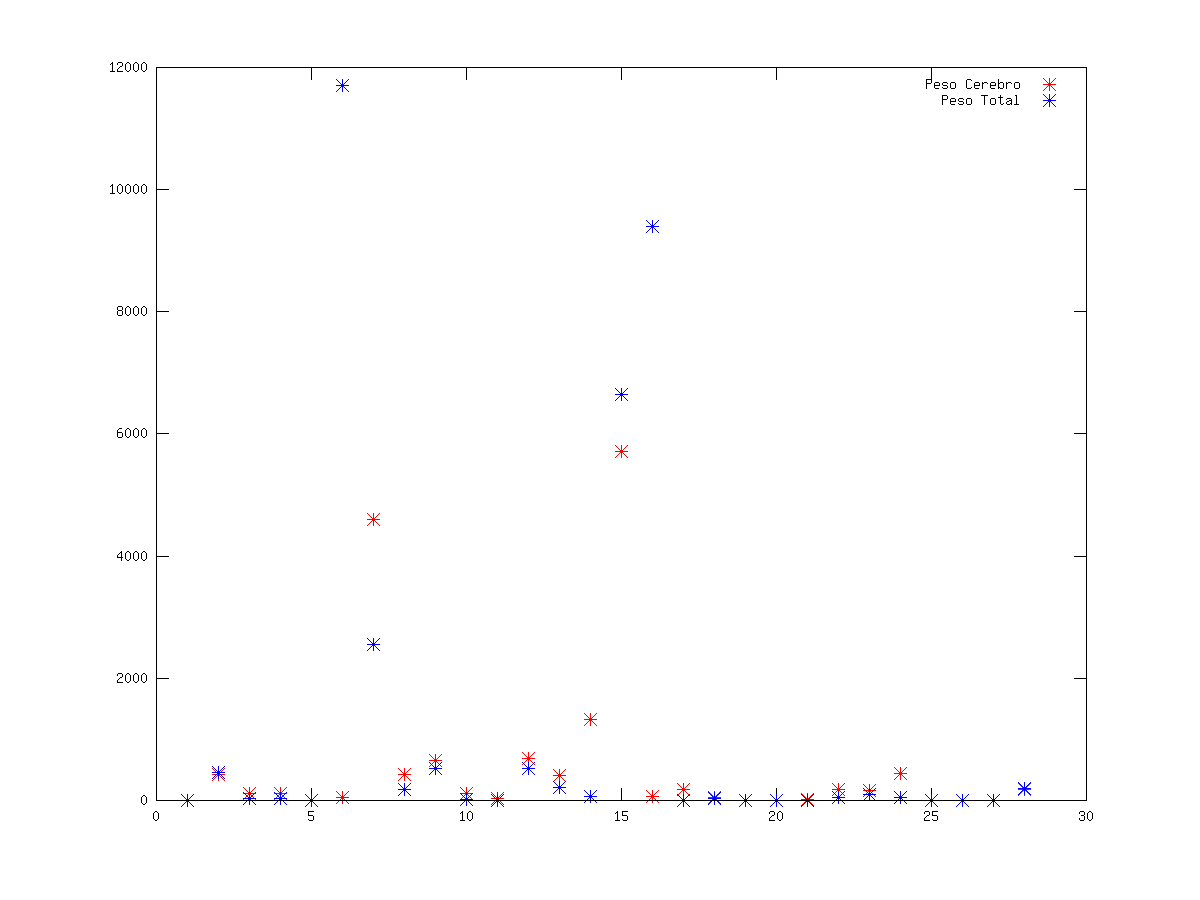
\includegraphics[scale=0.2]{TotalWeightVsBrainWeight}\caption{Peso del cerebro y peso total para cada medición en brains.txt{*}}
\end{figure}



{*} El valor del peso del cerebro de la medición 25 no se ve en la
figura ya que se aleja demasiado del resto de los valores y el ajustar
los ejes solo para mostrar ese valor produce que todas las demas mediciónes
no puedan apreciarse correctamente.


\begin{figure}[H]
\hspace{1cm}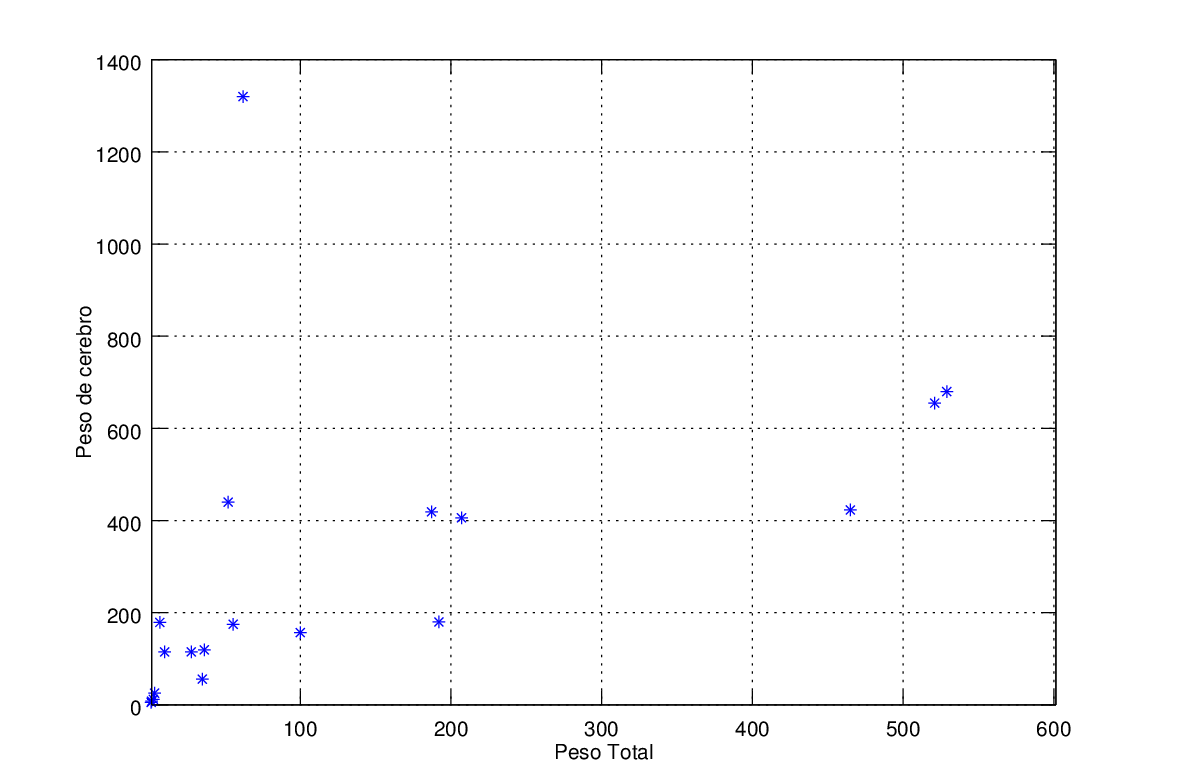
\includegraphics[scale=0.5]{TwVsBw}\caption{Peso total en Kg Vs peso del cerebro en G{*}{*}}
\end{figure}



{*}{*} Se removieron los valores para los $4$ valores de $x$ mayores
a $2000$ ya que ocultaban la visualización de todos los demás valores\\



En una observación a simple vista, se puede ver que las mediciónes
que se diferencian notablemente del resto son: $6,7,14,15,16$ y por
supuesto, la $25$.

\item No
\end{enumerate}
\item código

\begin{lyxcode}
load~brains.txt~

regstats(brains(:,1),~brains(:,2),'línear')

\begin{figure}[H]


\hspace{2cm}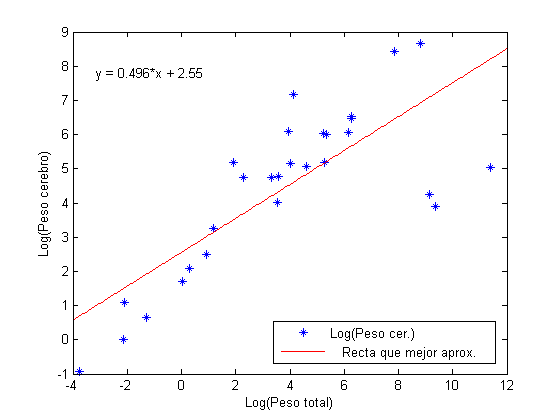
\includegraphics[scale=0.6]{logBrains}\caption{Logaritmo de ambas mediciónes y la línea que mejor los aproxima}


\end{figure}
\end{lyxcode}
\end{enumerate}
\end{enumerate}

\end{document}
